% Sample apostrophy’s to remove team's 

\title{Emergence of a Constructivist Grounded Theory Researcher: Grappling with a 2.5 Year Participant Observation Study }

\author{
\IEEEauthorblockN{ Todd Sedano }
\IEEEauthorblockA{Pivotal \\
  3495 Deer Creak Road \\
  Palo Alto, CA \\
  Email: professor@gmail.com}
}
% make the title area
\maketitle

\section{Abstract}
\textit{Context:} Conducting a Grounded Theory study is rigorous, demanding, and challenging. Misperceptions exist within the software engineering community \cite{StolGroundedTheory}.

\textit{Objective:} The purpose of this paper is to describe one extended participant observation Grounded Theory study for aiding new empirical researchers wanting to run similar research studies.

\textit{Method:} Following Constructivist Grounded Theory, we conducted a \durationOfResearchStudy{} participant-observation of \numberOfObservedProjects{} software development projects at Pivotal, a software development organization, interviewed \numberOfInterviews{} software engineers, interaction designers, and product managers, and analyzed one year of retrospection topics. We iterated between analysis and theoretical sampling until achieving theoretical saturation.

\textit{Results:}  This paper describes the mis-steps, challenges, and unique insights that occurred while conducting a grounded theory study.

\textit{Limitations:} While the process and results are highly relevant to the researcher, the outcomes might not apply to other researchers.

\textit{Conclusion:} Conducting my own Grounded Theory research study, attending Glaser’s Seminar, and reading and re-reading Charmaz’s and Glaser’s books helped the researcher overcoming misperceptions about Grounded Theory research.
\section{Introduction}

\participantQuote{Grounded Theory is such a simple method, yet so easily and often misapplied \cite{StolGroundedTheory}. It is easy to describe but hard to understand. My Grounded Theory study appears typical: confusion followed by insight. A researcher starts a Grounded Theory study open to see where the research leads. Once unleashed, the method seems to have a mind of its own as it guides the researcher towards research treasure through uncharted territory. I’ve been teaching and performing Extreme Programming for over 11 years, yet the method delighted me by finding precious insight}  \textemdash Todd Sedano \footnote{Interviewing oneself is an acceptable practice for participant observation in Grounded Theory even if it may seem like cheating}. 

For the past 2.5 years I've been conducting a full-time participant observation grounded theory study. Lengthy participant observation studies are unusual in software engineering and in computer science more generally. This paper describes my experiences in order to help future researchers considering a similar trajectory. 

My first introduction to Grounded Theory came while reading Bren\'{e} Brown’s \underline{Daring Greatly} \cite{BreneBrownDaringGreatly} in March 2013. Brown spends a significant portion of her book detailing her journey in applying Grounded Theory to her psychological research about into processing shame. Given my strengths with interpersonal communication, the technique appealed to me. 

While attending ICSE in San Francisco in May 2013, I participated in the first International Workshop on Conducting Empirical Studies in Industry (CESI 2013). I pestered researchers about how they used Grounded Theory in their research. (Thanks to Irit Hadar and Christopher Bull for answering all of my questions.) After the workshop, during the main conference, I sought out each Grounded Theory presentation to learn more about how the community used the method. I was hooked. 

Given the philosophical differences between the three variants of Grounded Theory, my co-advisor recommend that I examine and select one. Initially, I chose Constructivist Grounded Theory simply because it was the latest, a fine justification for selecting software libraries, but as I later discovered, not the best reason for selecting a sociological research method. 

I continue to use Constructivist Grounded Theory because it allows for the recording and transcription of interviews, enables literature review when appropriate in the research process, and builds upon decades of grounded theory research and experience. The philosophical stance of constructivism (as opposed to positivism) acknowledges the researcher's and participants' contributions to the construction of concepts. Positivistism acknowledges that knowledge from observable facts whereas constructivism posits that knowledge situated in a human context which may be more useful in understanding social interactions. For software engineering research, Constructivist Grounded Theory seems aptly suited since software development is a socio-technical endeavor.

Equipped with a copy of Charmaz’ Constructing Grounded Theory, I started my research study.

The purpose of this paper is to describe the evolution of both the researcher and the research study by examining phases of a 2.5 year Constructivist Grounded Theory study.  I divide the narrative into Section \ref{TheBeginning} \quotes{The Beginning,} Section \ref{TeamCodeOwnershipAndSustainableSoftwareDevelopment} \quotes{Team Code Ownership and Sustainable Software Development,} and Section \ref{RemovingWaste} \quotes{Removing Waste.}

\section{The Beginning}
\label{TheBeginning}
Following Glaser’s advice of \quotes{just do it} \cite{GlaserIssues}, I learned the intricacies of Grounded Theory while conducting my first Grounded Theory study. At each stage of the research, I read the next few chapters to understand what I would be doing next. My primary text was Charmaz \cite{Charmaz}, which I supplemented with Glaser’s books \cite{GlaserDiscovery, GlaserTheoreticalSensitivity, GlaserIssues} to build a deeper understanding of the method and the historical context of Constructivist Grounded Theory. 

This section presents the research context and explains why we selected Pivotal Labs. This section then describes the data collection and the data analysis at the beginning of the research study until core categories emerged.
\subsection{Research Context: Pivotal Labs}
\label{ResearchContext}
We selected Pivotal because: 1) it is successful; 2) it is interesting in its continued use and evolution of extreme programming; 3) it is accessible and cooperative with research. Both Classic and Constructivist Grounded Theory advocate picking an interesting site to see \quotes{What’s going on here?} 

Pivotal Labs is a division of Pivotal\textemdash a large American software company (with 17 offices around the world). Pivotal Labs provides teams of agile developers, product managers, and interaction designers to other firms. Its mission is not only to deliver highly-crafted software products but also to help transform clients' engineering cultures. To change the client's development process, Pivotal combines the client's software engineers with Pivotal's engineers at a Pivotal office where they can experience Extreme Programming \cite{BeckExtremeProgramming2004} in an environment conducive to agile development. Pivotal Labs has followed Extreme Programming \cite{BeckExtremeProgramming2004} since the late 1990's. 

\sout{\textit{Lessons learned: Considering your research site:} We found selecting a consultancy to be helpful as they were open to us researching the way they work provided we did not reveal information about the client.}
\subsection{Data Collection}
The research study started with data from two sources: 1) interviews with Pivotal employees and 2) participant observation. When I started data collection, I had no notion of the number of interviews or amount of participant observation that I would conduct. 
\subsubsection{Interviews}
The interviewees consisted of \numberOfInterviews{} interaction designers, product managers, and software engineers who had experience with Pivotal's software development process from five different Pivotal offices. 

Interview candidates were selected opportunistically. If a Product Manager from the New York office visited the Palo Alto office, I would attempt to schedule an interview that day. When I visited the Los Angeles area for a vacation, I scheduled interviews at the Santa Monica office.

I relied on \quotes{intensive interviews,} which are \quotes{open-ended yet directed, shaped yet emergent, and paced yet unrestricted} \cite{Charmaz}. Open-ended questions were used to enter into the participant's personal perspective within the context of the research question. The interviewer attempts to abandon assumptions to better understand and explore the interviewee's perspective. Charmaz \cite{Charmaz} contrasts intensive interviews with informational interviews (collecting facts), and investigative interviews (exposing hidden intentions, practices or policies).

The initial interviews were open-ended explorations starting with the question, \quotes{Please draw on this sheet of paper your view of Pivotal's software development process.} My goal was not to force initial topics and merely follow the path of the interviewee. In practice, the drawings provided a natural starting place for follow-up questions. Figure \ref{2015_08_12_simple} shows a simple drawing and Figure \ref{2015_08_12_detailed} shows a detailed drawing. 

I continued this approach until I wanted to explore emergent core categories as described in Section \ref{TeamCodeOwnershipAndSustainableSoftwareDevelopment}.

\begin{figure}[htbp]
\centering
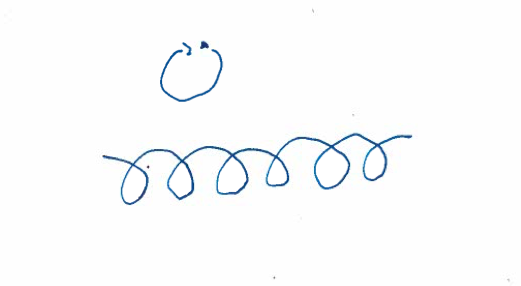
\includegraphics[width=\oneColumnWidth{}]{drawings/2015_08_12_se.png}
\caption{Interview 8: Simple drawing of Pivotal’s software development process}
\label{2015_08_12_simple}
\end{figure}

\begin{figure}[htbp]
\centering
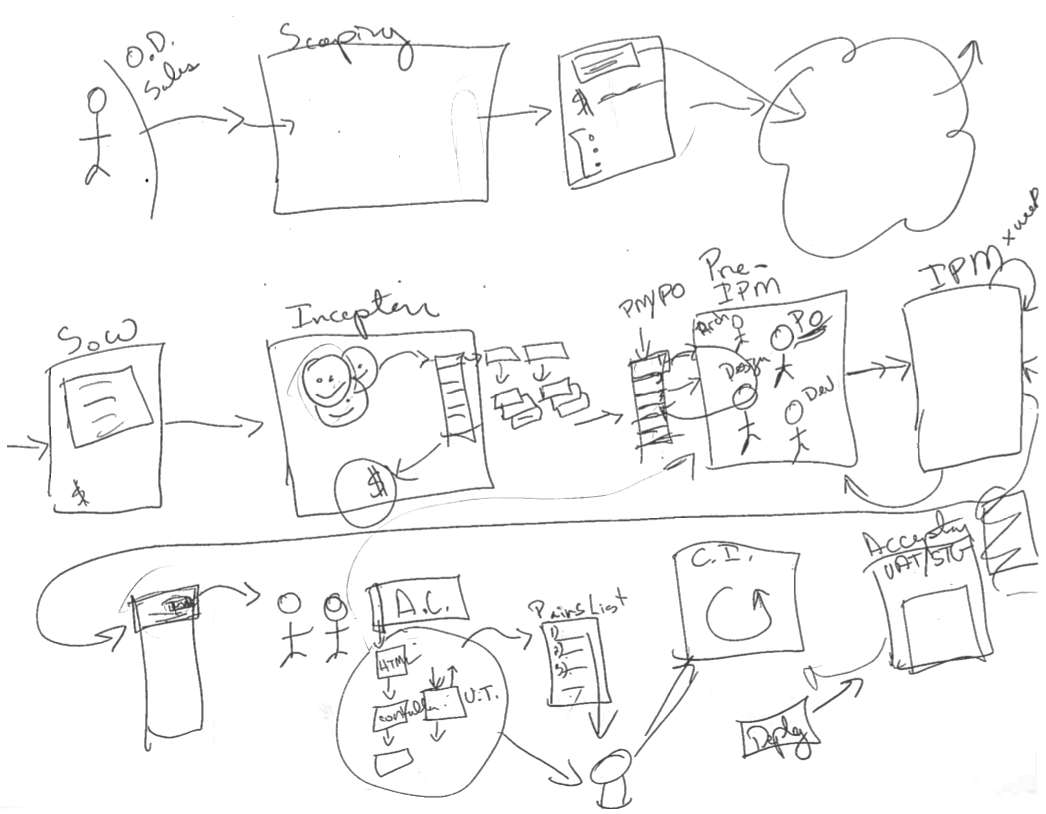
\includegraphics[width=\oneColumnWidth{}]{drawings/2015_08_12_anchor.png}
\caption{Interview 6: Detailed drawing of Pivotal’s Software Development process}
\label{2015_08_12_detailed}
\end{figure}
\subsubsection{Participant Observation}
While working as an engineer, I participated on \numberOfObservedProjects{} sequential projects lasting \durationOfResearchStudyPlural{} and collected field notes. These notes describe individual and collective actions, capture what participants found interesting or problematic, and include anecdotes and observations. Our waste taxonomy paper describes details about each project \cite{SedanoSoftwareDevelopmentWaste}.

Here is a portion of a field note: 
\participantQuote{Monday was the first time we started getting data from the client’s servers. We've been implementing for several months without knowing whether our system would work with real backend systems. In order to make progress, we created mocks for each of the client’s systems based upon documentation. Now we need to modify our code base to match the reality of the systems’ implementation.}
\subsection{Data Analysis}
Data analysis began by iteratively collecting and analyzing interview transcripts and participant observations. I used line-by-line coding \cite{Charmaz} to identify nuanced interactions in the data and avoid jumping to conclusions. My advisor reviewed the initial codes while reading the transcripts and listening to the audio recordings.  We discussed the codes and the coding process during weekly research collaboration meetings. To avoid missing insights from these discussions \cite{GlaserTheoreticalSensitivity}, we often recorded and transcribed the discussion into Grounded Theory memos. As data was collected and coded, I stored initial codes in a spreadsheet and I used constant comparison to generate focused codes.

I routinely compared new codes to existing codes to refine codes and eventually generate categories. I periodically audited each category for cohesion by comparing its codes. When this comparison became complex, I printed codes on index cards, and then arranged and re-arranged until cohesive categories emerged. I wrote memos to capture the analysis of codes, examinations of theoretical plausibility, and insights.

I attended Glaser’s Grounded Theory Seminar in Mill Valley, CA. Glaser structures the workshop to help aid the attending researchers to move from their current phase to the next phase of the Grounded Theory process, not transition them to the final step. Glaser intentionally a challenges participant’s point of view. From his perspective, an attendee having an emotional breakdown would be a sign of a successful workshop.


\participantQuote{Just before my time, I changed my question for him. Before me, he tore into someone for bringing pre-conceived notions to the research. I'm kicking myself for not being true to my original question, although at the time I was rationalizing it by trying to incorporate everything that I was learning. This is something that I can grow through, the \quotes{shoulda, woulda, couldas.}} \textemdash My email notes to advisor.

Here’s a personal memo from my experience, \participantQuote{I’m discouraged. I regret that I panicked. I didn’t want to be taken apart like the lady from Trinidad and Tobago. So, I am sad. It would be nice for an “awesome” theory to emerge from this work. I feel like a failure. I wish this was not the case as I’m very happy with the work that I have done. I am very glad to have a deeper understanding of Glaser’s approach (since it is so hard to reverse engineer it from his books.) I’m also afraid that if I start asking engineers \quotes{how is your day going} and \quotes{what is on your mind} that I’ll get a lot of technical jargon that will be difficult to group into a pattern.}

The workshop helped me understand the fundamental terms used in Grounded Theory. At the time, I was reading through three of Glaser’s books \cite{GlaserDiscovery, GlaserIssues, GlaserTheoreticalSensitivityLong} since I was struggling to understand constant comparison and the conversion of codes into categories. These books do not clearly define the terms; distinguish the differences between the terms; nor provide clear examples illustrating the concepts. Listening to Glaser discuss the concepts helped me solidify what he meant by each term. Later, I discovered that his book \cite{GlaserBasics} does define the terms in response to the Strauss and Corbin book \cite{Strauss1988Basics}.

Finding a candidate structure that supported and explained the data took time. For a while, the data was fractured around many different topics and I struggled to integrate the data into a cohesive whole. I tried rotating and pivoting the data through different lenses. Glaser said that \quotes{confusion is the royal road to emergence,} \cite{GlaserMillValleyWorkshop} and confusion appears to be a typical, critical step for the Grounded Theory researcher. Eventually, I had my ah-ha moment when I found a candidate structure that explained the data at different levels of software development. 

Focusing Grounded Theory on one category helped me make forward progress. When I reviewed the candidate structure with my committee, I expressed my concern about its publishability. A model of course correcting was potentially not interesting to the software engineering community, as several people have already discussed feedback loops. Since I had not fully written memos describing the emerging theory, I had difficulty in explaining the structure to my committee. Sensing that perhaps I had taken on too much with my first Grounded Theory study, my co-advisor suggested that I focus on one concrete category. In retrospect, this advice proved beneficial as I learned Grounded Theory on a focused topic which allowed me to make forward progress in performing constant comparison and working through theoretical sampling.

Thus, I pivoted my interviews and data collection on \quotes{code ownership,} one of the categories in my course correcting theory. This decision transitioned me to the second phase of the Grounded Theory study.
\section{Team Code Ownership and Sustainable Software Development}
\label{TeamCodeOwnershipAndSustainableSoftwareDevelopment}

Focusing the research study on \textit{code ownership}, one of the categories, changed the interviewing process to explore this topic, focused constant comparison, and began theoretical sampling. 

\subsection{Data Collection}
I continued to initiate Interviews with open-ended questions. Now I asked participants, \quotes{please draw your feelings about the code} which often resulted in conversations about code ownership. Figure \ref{Interview31} and Figure \ref{Interview32} are examples from this phase of the research study. 

\begin{figure}[htbp]
\centering
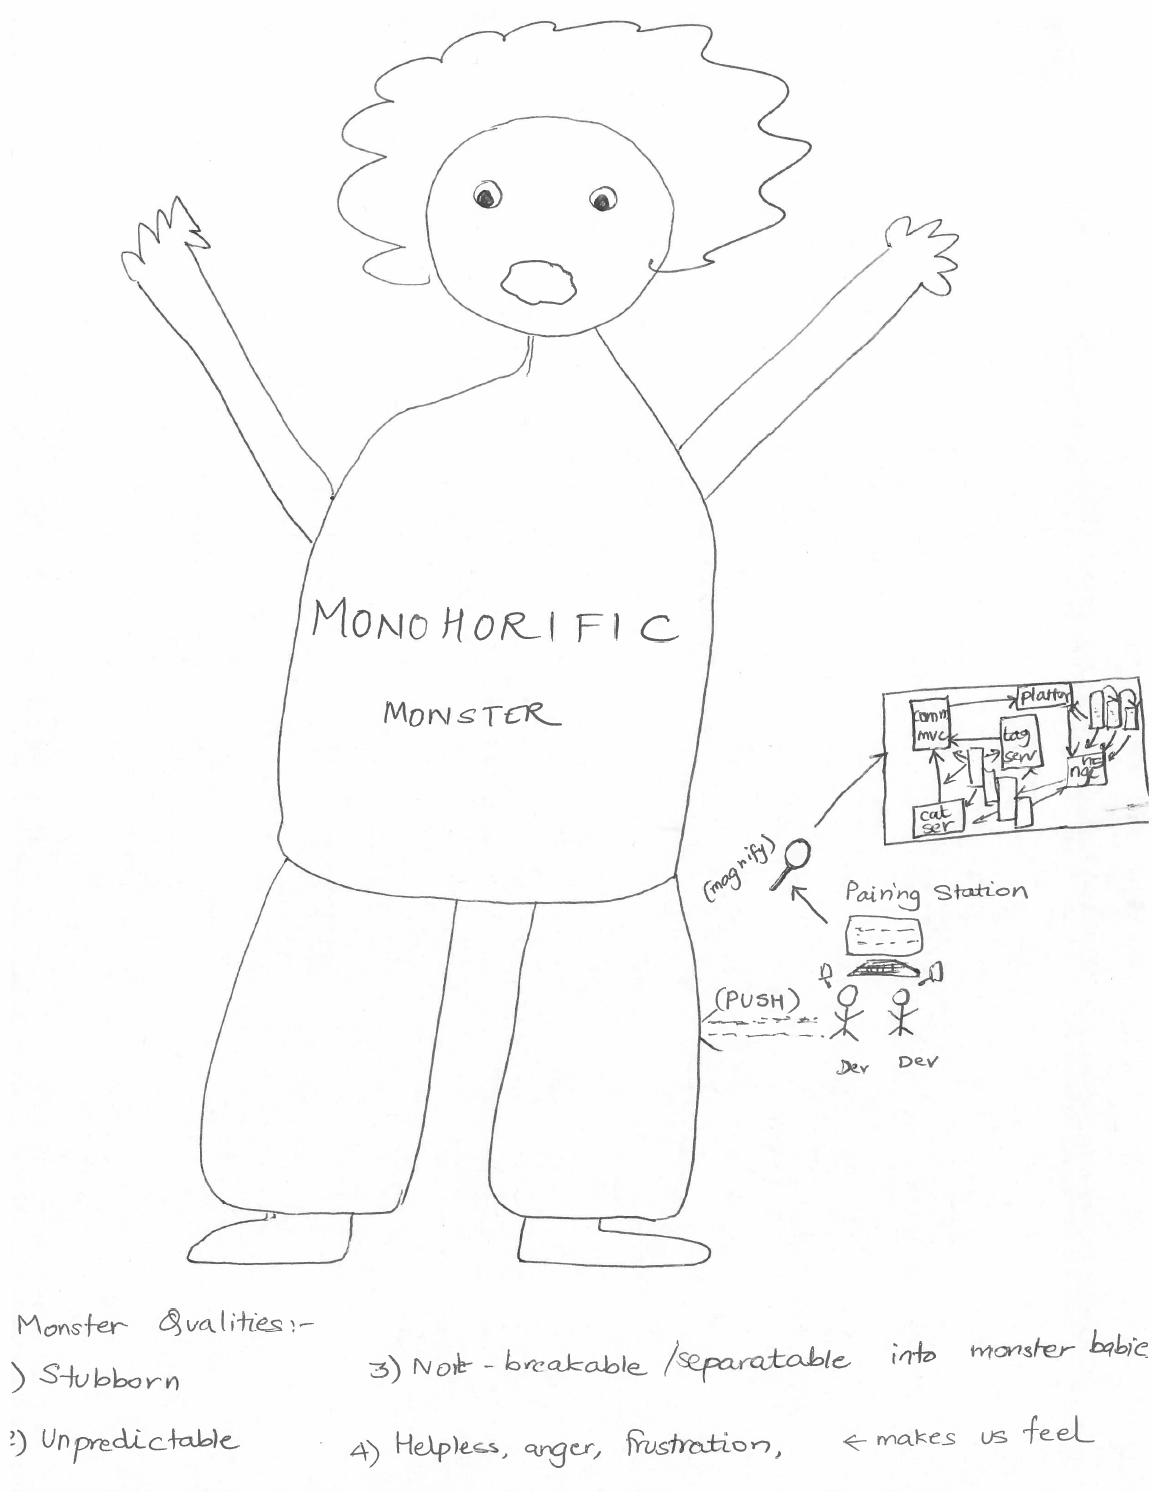
\includegraphics[width=\oneColumnWidth{}]{drawings/2016_09_26.png}
\caption{Interview 31: Software Engineer's drawing for \quotes{How you feel or how you think about the code'}}
\label{Interview31}
\end{figure}

\begin{figure}[htbp]
\centering
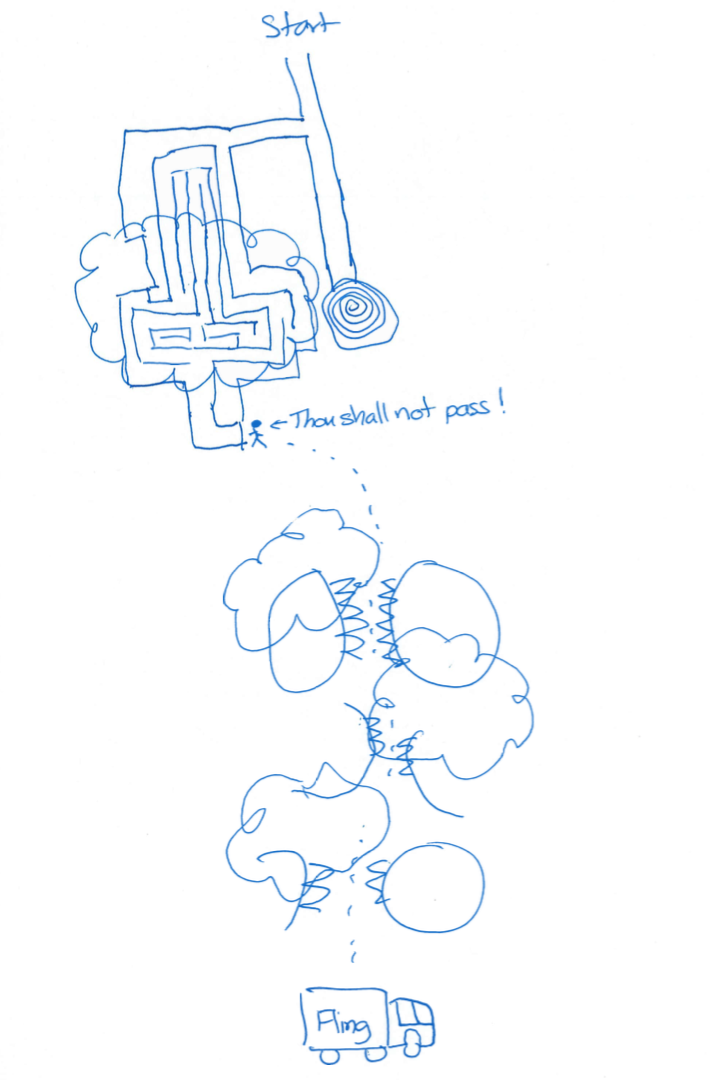
\includegraphics[width=\oneColumnWidth{}]{drawings/2016_09_29.png}
\caption{Interview 32: Software Engineer's drawing for \quotes{How you feel or how you think about the code}}
\label{Interview32}
\end{figure}

I continued participant observation, collecting examples of when team actions affected code ownership. 

\subsection{Data Analysis}
Two interrelated concepts emerged from the Grounded Theory analysis: team code ownership and sustainable software development. Identifying and disentangling them was not easy and the remainder of this Section \ref{TeamCodeOwnershipAndSustainableSoftwareDevelopment} is devoted to that process.

\textbf{Team Code Ownership}

The analysis (coding the interviews, performing constant comparison for code ownership, and writing memos) revealed that the emerging idea expanded beyond Beck’s \cite{BeckExtremeProgramming1999, BeckExtremeProgramming2004} and Fowler’s \cite{FowlerCodeOwnership} idea for collective ownership and collective code ownership. The prior literature described collective code ownership as a policy statement, where teams would decide who could modify which parts of the code. In contrast with individual code ownership where one programmer owns a set of files, collective code ownership allowed anyone to modify any part of a system. I observed events that weakened a team’s sense of ownership of the code. The team’s sense of ownership was dynamic. I was analyzing something new. 

I struggled with what to name the emerging idea. Is the emergent idea a modification of collective code ownership or is it fundamentally a different concept? My memos reflect the  journey of looking for an apt term: \quotes{I’m looking for a term that describes the relationship between the developer and their sense of ownership of the code.} My memos contain a progression from \quotes{code ownership} to \quotes{communal code ownership} to \quotes{collective code possession} to \quotes{team code ownership.} 

We resolved the tension by defining a new term and differentiating it from collective code ownership. We defined team code ownership as \quotes{the ability for any developer on a team to change any of the team’s code.} A team could decide to adopt collective code ownership and exhibit other behaviors (such as implementing hard to understand code or ostracizing a team member) that would make it challenging for a developer to modify the team’s code. Fortunately, we could not find any published work using or defining team code ownership.

As the ideas of code ownership began to solidify, I started reviewing the literature looking for how papers grappled with the idea of ownership. A paper on psychological ownership \cite{Pierce2001} allowed me to connect the deep human needs that fuel our need for ownership with team code ownership and explained how psychological ownership affects our transition from individual code ownership to team code ownership.

For a long time during analysis, the dividing line between Team Code Ownership and Sustainable Software Development was unclear. Teasing apart these concepts was challenging, in part, because each concept had no clear name. 

% My ideal name was an \textit{in vivo} code, one generated from the participants. Two months earlier, during an interview, I originated the phrase \quotes{team code ownership} when I summarized what the interviewee said back to the interviewee. As a participant observer, I had labeled the concept in a way that resonated with the participants.

% \quotes{What I am describing is more than a policy about if you can or cannot modify the code. If you read the agile alliance's definition of code collective ownership it's similar to Québec's approach which is simply a policy statement.}


\textbf{Sustainable Software Development}

Participant observation enabled a crucial insight. One day as I was pair programming, I realized that I did not know who was on my team. Why? The team suffered from significant team churn. I wondered who had worked on the project. During my Christmas break, I converted the allocation data into a chart listing the start and stop dates for each team member. The graph surprised me. How was it possible to be successful \cite{RalphDimensionsOfSuccess} with the client with so many people rotating through the project? By following certain practices, the team thrived through disruptive events.

However, the one insight would require significant analysis to tease apart the Theory of Software Development. 
\subsection{Theory Construction and the Emergence of a Theoretical Family}
The emergence of the relationship between team code ownership and sustainable software development required many iterations. 

Labelling the idea that emerged from the analysis through constant comparison and memo writing proved problematic. Through the memoing process, I grappled with the ideas of code ownership and its relationship with an abstract idea that the team could thrive through team churn. While I knew that the two were related from the data, initially it was opaque to me where one stopped, the other started, and what to call each idea. My process for solving this tension looked like this:

\begin{enumerate}
  \item Be confused
  \item Try a relationship between the categories
  \item Iterate on Step 2
  \item Experience an \quotes{Ah ha} moment
  \item Verify with data
\end{enumerate}

I tried looking at parent-and-child relationships. Did ownership cover both ideas? No. Did the surviving team churn concept cover both ideas? Maybe. I tried sibling relationships. Were the two concepts equal to each other with an over arching idea comprising them?  No. I reviewed the 18 theoretical coding families in Glaser’s \underline{Theoretical Sensitivity} \cite{GlaserTheoreticalSensitivity}. In time, my advisor and I labeled the surviving team churn category, \quotes{sustainable software development} with team code ownership as one of its properties. 

We then started teasing apart the relationships between all the subcategories. Several felt different from each other. In time, we realized that some were practices, some were policies, and some were underlying principles. 

Refining the practices into logical groups was hard. Articulating what is in the researcher’s head can be difficult. We had identified six practices that supported sustainable software development by supporting team code ownership. We wondered if we could separate them into groups. My advisor proposed a separation based upon my advisor’s expert opinion from reading the interview transcripts. The proposal did not resonate with me as the participant observation data did not entirely support it. The proposal spurred me into reconsidering the relationships between categories, much like when an editor is compelled to rewrite a poorly written sentence. I tried bifurcating the practices based on a series of questions. The question that worked for the data was, \quotes{which of these practices differently affects the code?} Three of them did. Then I asked \quotes{how are these other practices related?} Oh, they all touch on knowledge silos. I recalled two interviews. One interviewee discussed caretaking the code like a gardener. Another interviewee discussed concern about knowledge silos forming on the team. I then labeled each group with \textit{in vivo} codes. This process is how we discovered the \quotes{Caretaking the Code Practices} and \quotes{Removing Knowledge Silos Practices} categories. 

In Grounded Theory, the researcher must sit with uncomfortableness of the process. When in doubt, gather more data and continue constant comparison. In time, the brain will solve the problem find order in the chaos 

Through iterations, the structure of the Theory of Software Development arrived. Sometimes emergence of the theoretical structure takes time.

I found that working with an idea without a label challenging, but rewarding. 

Once the theory emerged, the question arose: \quotes{what more data do I need to collect?} and \quotes{is this good enough for publication? }
\subsection{Theoretical Saturation}
Theoretical sampling is collecting additional data to develop full and robust categories, identify the relationships between categories, and flush out the main category’s properties.

Starting this research study, I thought I understood theoretical saturation. Eventually I realized that I did not, and I struggled to understand the concept. 

There’s a subtle distinction between “sampling until no new data emerges” and sampling to flesh out the emerging theory. In discussing theoretical sampling or “saturation” with software engineering researchers practicing Grounded Theory at ICSE 2013, I misconstrued theoretical sampling as the continued collection of data until no new data and thus no new insights emerge. Stopping the process is logical if the collection of data results in the same kind of information. However, theoretical sampling has a subtle distinction from this misconception. Grounded Theory is not about asking the same questions over and over again until the same questions result in no new information. Grounded Theory alters the questions in response to the emerging data, and the researcher continues to ask new questions to help fill in the emerging theory. Thus, theoretical sampling is collecting new information to illicit the relationship between codes, between codes and categories, and between categories. The process stops once the researcher has matured the theory as there is nothing more to ask the participants since there are no more questions to be answered.

At one point, I asked my advisor and co-advisor, \quotes{what questions should I ask my participants to achieve theoretical saturation?} In retrospection, this was an unfair question. As the primary researcher, I know the data the best, and I am the one most qualified to know which relationships between the categories are not robust. Although I did not realize it at the time, I was \textit{already} asking questions to better understand the emergent theory. In essence, I wanted my advisors to bless my results and let me know that I was doing the process correctly, instead of relying on the emergence from the data.

I shifted the question from \quotes{what questions will get me theoretical saturation?} to asking myself, \quotes{what do I not know about this theory?}, \quotes{what is confusing?}, and \quotes{how do each of these categories relate?}

I finally understood Theoretical Saturation by re-reading Charmaz and Glaser many, many times. 


In summary, the data advanced from the initial codes to focused codes, focused codes to core categories, and core categories to an emergent theory. 

Resulting in two papers\cite{SedanoSustainableSoftware, SedanoTeamCodeOwnership}/

\section{Removing Waste}
\label{RemovingWaste}

When \textit{removing waste} appeared as a core category, we began collecting and analyzing data from retrospectives. We continued to collect participant observation data and continued interviewing until achieving theoretical saturation. 



\subsection{Data Collection}
\subsubsection{Retrospection Topics}
A retrospection meeting (or retro) is a weekly meeting to pause, reflect, and discuss the work done during the week, i.e., a safe place where any team member can discuss any issue \cite{DerbyAgileRetrospectives}. Retros are typically scheduled every Friday afternoon. The entire team and important stakeholders attend these meetings. 

The observed Pivotal teams mostly use an emotion-based retro format where \quotes{happy,} \quotes{meh,} and \quotes{sad} faces are written on the top of a whiteboard. The happy-face column represents items that are working well, of which the team wants to do more. The meh-face column represents  items that the team needs to \quotes{keep an eye on.} The sad-face column represents items that need improving, which the team should try to fix. Any team member can add any topic to any column. After a few minutes, the team dot-votes on the topics to discuss \cite{DerbyAgileRetrospectives}. The team uses the remainder of the sixty-minute meeting to discuss topics. Sometimes discussing a topic is sufficient to affect change, other times the team creates action items. 

We collected data from 91 retrospection meetings. After removing irrelevant topics (e.g. complaints about the weather), we printed each retro item onto an index card with its original retro topic, enhanced description, id, and team name (see Figure \ref{exampleRetroTopicl}).

For co-located teams, a whiteboard picture taken at the end of the retro was later transcribed into a master spreadsheet. For distributed teams, we copied data from on-line spreadsheets that the team used in-place of a whiteboard. Attendees often wrote a short phrase as a proxy for a larger idea. For example, \quotes{Scope} represents \quotes{Too much scope is causing the team stress} or \quotes{Legal} represents \quotes{Waiting on legal to approve the legal web pages.} When the provided topic was too vague, we solicited a more detailed description from an engineer present in the meeting. This produced 663 total items for analysis. 

\begin{table}[t]
\renewcommand{\arraystretch}{1.5}
\centering
\captionof{figure}{Example Retro Topic Index Card }
\label{exampleRetroTopicl}
\begin{tabular}{|l|}
\hline
Topic: Legal \\ \\ Description: Waiting on Legal to approve legal pages \\ \\ Id: 182 Project: Quattour\\ \hline
\end{tabular}
\end{table}
\subsection{Data Analysis}
Over the course of two days, two researchers with first-hand experience of the projects did initial coding of the retro topics and merged duplicate topics. We rearranged initial coding categories to be near similarly themed categories and iteratively combined and reorganized categories. We often stopped to record new insights as memos. When the categories began to stabilize, we compared each category against the other categories looking for relationships. Once we felt that the categories were stable, we performed a review of each category to verify that the cards belonged to it, creating a first draft of the waste taxonomy.

Just because a topic made it to the \quotes{needs improvement} column of a retro did not meant that it was a software development waste. Some topics were just complaints.

Participant observation provided the needed context for understanding the retro data. The short phrases written on a whiteboard did not provide enough context for understanding the underlying issue and potential waste. By experiencing the projects with the participants enabled me to reason about the issues. 

The analysis process revealed that answering the question, \quotes{is this topic a waste?} was no simple task. Often all three co-authors discussed if a topic was a waste type or a cause of waste. On one occasion, I longed to have a waste taxonomy as simple and well defined as the well-established Toyota Production System waste taxonomy. I noticed that the manufacturing waste of \textit{overproduction} created \textit{inventory} waste. Realizing that the accepted manufacturing waste taxonomy double counts one wasteful cause as two types of waste, reminded me that balancing simplicity with accuracy is challenging. 

We continued theoretical sampling for team code ownership and removing waste in additional interviews and participant observations until no further waste-related categories were evident, i.e. theoretical saturation. 

On one project, the backlog routinely had blocked stories at the top of the backlog. On other projects, the Product Manager would move blocked stories to the icebox and then reprioritize the stories into the backlog when ready. Since blocked stories at the top of the backlog may be unusual, sometimes developers would begin working on a story before realizing that the story had a \quotes{blocked} label on it. Quickly, the developers learned to skim down the list of next stories to find the first ready story to work on. The developers complained about this inefficiency during a retro. Clearly starting and stopping stories is inefficient. I wondered if blocked stories were a waste in and of themselves. In follow-up interviews with Product Managers, I ascertained that waiting for information is a normal part of Product Managers’ workflow as they try and prepare a story for readiness. A Product Manager handles context switching of information so that the engineers have ready-to-work-on-stories. For the Product Manager, there can be natural waiting waste. Blocked stories are not a symptom of a larger problem on the team.
In summary, the data advanced from the initial codes to focused codes, focused codes to core categories, and core categories to an emergent theory. 

Resulting in \cite{SedanoSoftwareDevelopmentWaste}.
\section{Evolution of materials}
Over the course of this research study, the tools that I used for constant comparison evolved. I now prefer using tactile manipulatives over electronic storage. 

Here is my experience:
\begin{enumerate}
  \item I initially did all constant comparison in google spreadsheets
  \item I started hand-writing cards for hard-to-understand or complex comparisons and I would physically sort them around me in a circle (e.g. needing to make sense of multiple perspectives about a backlog)
  \item I printed the codes directly related to team code ownership onto index cards
  \item I printed all the retrospective notes onto index cards
\end{enumerate}

The advantages of electronic storage include:
\begin{itemize}
  \item Available wherever you have a computer
  \item Easy to share with co-authors
  \item Easy to backup and duplicate
  \item Simple to turn into physical cards
\end{itemize}

The advantages of physical medium include:
\begin{itemize}
  \item Easy to rearrange
  \item Easy to see big picture 
  \item Easy to focus on one area
  \item Easy to see outliers
  \item Easy to annotate with thoughts
  \item Encourages short capturing of ideas
  \item Time consuming to turn into electronic storage
\end{itemize}

Holding a card typically forces me to consider it before I put it down. When looking at rows in a spreadsheet, they tend to blur together and it's easier for me to gloss over them. When I see rows near each other in a spreadsheet there is a subconscious implication that they belong together. Picking up the next physical card implies that it is something new. 

I enjoy the sound of ripping up index cards when they have evolved or are no longer relevant

For the waste taxonomy I maintained \textit{both} an electronic and physical copy which was time consuming and felt wasteful. For my next study, I’m planning on coding using Microsoft Word, converting the codes into a Microsoft Excel spreadsheet for printing onto index cards. I would then manage index cards until the camera ready version of the paper is submitted. Finally, I would update the code’s categories in Excel for archival purposes.

Grounded Theory researchers discovers what techniques work for them. 
\section{Conclusion}
As documented by Stol et al \cite{StolGroundedTheory} common misperceptions exist in software engineering literature about Grounded Theory. By describing my own journey, I hope that the next generation of Grounded Theory researchers can learn from my experience. 

For me, understanding the core terms, \quotes{codes} and \quotes{categories} 

Theoretical saturation is collecting additional data to develop full and robust categories, not collecting additional data until nothing new emerges. Theoretical sampling pivots the data collection process to collect missing information. 

My thinking evolved from \quotes{I have access to this data, what do I do with it?} to \quotes{given this participant’s concern or observation, how do I get the data to flesh out the idea?}

I have evolved my Grounded Theory process from using of electronic tools for constant comparison to using physical index cards.

Each Grounded Theory might follow a path of confusion followed by insight. Finding a clarifying question may help position the analysis, however this question is unique to the study’s confusion.

Glaser says that a Grounded Theory study can create a rich trove of data. I am still analyzing the data and look forward to the next papers to come from this research study.















